\documentclass[12pt]{article}
\usepackage{amsmath, amssymb, amsthm}
\usepackage{enumitem}
\usepackage{xcolor}
\usepackage{tikz}

\title{Section 5.1.2 – The Principle of Mathematical Induction}
\author{SWOSU Discrete Structures}
\date{}

\begin{document}
\maketitle

\section*{The Principle of Mathematical Induction}

Mathematical induction is like proving that a line of dominoes will all fall over.  
To show this:
\begin{enumerate}
    \item You knock over the \textbf{first domino} (the \textbf{basis step}).
    \item You show that \textbf{whenever one domino falls}, it knocks over the next (\textbf{inductive step}).
\end{enumerate}

\noindent Once those two steps are shown, every domino falls, every ladder rung is reached, and every integer gets its proof hug.  

\vspace{1em}
\noindent Expressed formally:

\[
\big( P(1) \wedge \forall k (P(k) \rightarrow P(k+1)) \big) \rightarrow \forall n\, P(n)
\]

\section*{Try It Yourself}

\textbf{Statement:} $1 + 3 + 5 + \dots + (2n - 1) = n^2$

\begin{enumerate}[label=\alph*)]
    \item \textbf{Base Case:} Prove the formula works when $n=1$.  
    \vspace{1em}
    \item \textbf{Inductive Hypothesis:} Assume the formula works for some $k$.  
    \vspace{1em}
    \item \textbf{Inductive Step:} Prove it works for $k+1$ by using your hypothesis.  
    \vspace{1em}
    \item \textbf{Conclusion:} What does this mean for all positive integers $n$?
\end{enumerate}

\section*{Historical Note}

The method dates back to the 1500s with Francesco Maurolico — a mathematician who proved things before proofs were cool.  
He showed, for example, that the sum of the first $n$ odd integers equals $n^2$ (yep, the problem you just did).

\section*{Visual Thinking Challenge}

Draw a quick sketch of dominoes labeled 1 through 6.  
Show which two statements ($P(1)$ and $P(k)\rightarrow P(k+1)$) guarantee the entire chain falls.

\vfill
\begin{center}
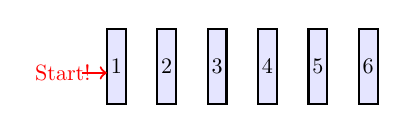
\begin{tikzpicture}[scale=0.8, every node/.style={scale=0.8}]
    \foreach \x in {1,...,6}{
        \draw[fill=blue!10, thick] (\x*0.8,0) -- ++(0.3,0) -- ++(0,1.2) -- ++(-0.3,0) -- cycle;
        \node at (\x*0.8+0.15,0.6) {\x};
    }
    \draw[->, thick, red] (0.4,0.5) -- (0.8,0.5);
    \node[red] at (0.1,0.5) {Start!};
\end{tikzpicture}
\end{center}

\end{document}

